\chapter{Schroedinger equation in 3d}
\label{chap:sch_3d}

After we have considered two-dimensional Schroedinger equations, we are now ready for
the extension to three-dimensional systems. In 3d, Schroedinger equation can be
written as:
\begin{equation}
\left[ -\frac{1}{2}\nabla^2 + V(\mathbf{r}) \right] \psi(\mathbf{r}) = E\,\psi(\mathbf{r})
\end{equation}
where $\mathbf{r}$ is the abbreviation to $(x,y,z)$ and
%
$\nabla^2$ is the Laplacian operator in 3d:
\begin{equation}
\nabla^2 = \frac{\partial^2}{\partial x^2} + \frac{\partial^2}{\partial y^2} +
\frac{\partial^2}{\partial z^2}
\end{equation}

\subsection{Three-dimensional grid}

As in the preceeding chapter, our first task is to create a representation of 3d grid
points and various quantities defined on it. This task is realized using straightforward
extension of \txtinline{FD2dGrid} to \txtinline{FD3dGrid}.


Visualization of 3d functions as isosurface map or slice of 3d array.

Introducing 3d xsf


\subsection{Laplacian operator}

The Laplacian in 3d can be written as:
\begin{equation}
\mathbb{L} = \mathbb{D}^{(2)}_{x} \otimes \mathbb{I}_{y} \otimes \mathbb{I}_{z} +
\mathbb{I}_{x} \otimes \mathbb{D}^{(2)}_{y} \otimes \mathbb{I}_{z} +
\mathbb{I}_{x} \otimes \mathbb{I}_{y} \otimes \mathbb{D}^{(2)}_{z}
\end{equation}

The Julia code is also similar to the one we have used for the case of 2d:
%
\begin{juliacode}
const ⊗ = kron
function build_nabla2_matrix( grid )
  # ... SNIPPED
  # build D2x, D2y, and D2z matrices
  IIx = speye(grid.Nx)
  IIy = speye(grid.Ny)
  IIz = speye(grid.Nz)    
  ∇2 = D2x⊗IIy⊗IIz + IIx⊗D2y⊗IIz + IIx⊗IIy⊗D2z
  return ∇2
end
\end{juliacode}
%
The main difference is that we have used the symbol \txtinline{⊗} in place
of \txtinline{kron} function to make our code simpler. In Julia this symbol
can be entered by typing \txtinline{\otimes} in Julia console or text editors
that have been set up to use Julia extension and Unicode input.


\section{3d harmonic oscillator}

We hope that at this point you will have no difficulties to create your own
Schroedinger equation solver for 3d harmonic potential:
\begin{equation}
V(x,y,z) = \frac{1}{2}\omega^2 \left( x^2 + y^2 + z^2 \right)
\end{equation}

The analytic solution for the energy levels of this potential can be written as:
\begin{equation}
E_{n_{x} + n_{y} + n_{z}} = \hbar \omega \left( n_{x} + n_{y} + n_{z} + \frac{3}{2} \right)
\end{equation}
where $n_x, n_y, n_z$ are integers positive integers including zero.
%
For each energy level we have the following degeneracies:
\begin{equation}
g_{n} = \frac{(n + 1)(n + 2)}{2}
\end{equation}
where $n = n_x + n_y + n_z$.
%
For examples:
\begin{textcode}
n = n_x + n_y + n_z

n = 0: (1)(2)/2 = 1  (E=1.5)
n = 1: (2)(3)/2 = 3  (E=2.5)
n = 2: (3)(4)/2 = 6  (E=3.5)
\end{textcode}

The following is the result of \jlinline{diag_Emin_PCG}, for the 4 lowest eigenstates:
\begin{textcode}
CG step       12 =       8.9999996162 4.4341014e-06
evals[  1] =       1.4999999732, devals =   4.1020002284e-07
evals[  2] =       2.4999998628, devals =   1.0054977597e-06
evals[  3] =       2.4999998760, devals =   1.3278320172e-06
evals[  4] =       2.4999999042, devals =   1.6905715712e-06
iter 12 nconv = 4
Convergence is achieved based on nconv    
\end{textcode}
%
The obtained eigenvalues are close the the analytic solution.
Note that the we have second lowest eigenstate of degeneracy 3.
You can try to vary the number of requested eigenstates to very that the degeneracies are
correct.


\section{Hydrogen atom}

\subsection{Coulomb potential and its singularity}

Until now, we only have considered simple potentials such as harmonic potential. Now we will
move on and consider more realistic potentials which is used in practical electronic calculations.

For most applications in materials physics and chemistry the external potential that is
felt by electrons is the Coulombic potential due to atomic nucleus. This potential has
the following form:
\begin{equation}
V(r) = -\sum_{I}^{N_{\mathrm{atom}}} \frac{Z_{I}}{\left|\mathbf{r} - \mathbf{R}_{I}\right|}
\end{equation}
where $R_{I}$ are the positions and $Z_{I}$ are the charges
of the atomic nucleus present in the system.
%
We will consider the most simplest system, namely the hydrogen atom $Z_{I}=1$, for which we have
\begin{equation}
V(r) = -\frac{1}{\left|\mathbf{r} - \mathbf{R}_{0}\right|}
\end{equation}
%
The following Julia code implement the H atom potential:
\begin{juliacode}
function pot_H_atom( grid; r0=(0.0, 0.0, 0.0) )
  Npoints = grid.Npoints
  Vpot = zeros(Npoints)
  for i in 1:Npoints
    dx = grid.r[1,i] - r0[1]
    dy = grid.r[2,i] - r0[2]
    dz = grid.r[3,i] - r0[3]
    Vpot[i] = -1.0/sqrt(dx^2 + dy^2 + dz^2)
  end
  return Vpot
end
\end{juliacode}

With only minor modification to our program for harmonic potential, we can solve the Schroedinger
equation for the hydrogen atom:
\begin{juliacode}
grid = FD3dGrid( (-5.0,5.0), Nx, (-5.0,5.0), Ny, (-5.0,5.0), Nz )
∇2 = build_nabla2_matrix( grid )
Vpot = pot_H_atom( grid )
Ham = -0.5*∇2 + spdiagm( 0 => Vpot )
prec = aspreconditioner(ruge_stuben(Ham))
Nstates = 1  # only choose the lowest lying state
Npoints = Nx*Ny*Nz
X = ortho_sqrt( rand(Float64, Npoints, Nstates) ) # random initial guess of wave function
evals = diag_LOBPCG!( Ham, X, prec, verbose=true )
\end{juliacode}

For the grid size of $N_{x}=N_{y}=N_{z}=50$ and using 9-point finite-difference approximation
to the second derivative operator in 1d we obtain the eigenvalue of -0.4900670759 Ha which
is not too bad if compared with the exact value of -0.5 Ha. We can try to increase the grid
size until we can get satisfactory result.

Note that there is a caveat when we are trying to use the Coulombic potential. This potential
is divergent at $r=0$, so care must be taken such that this divergence is not encountered in
the numerical calculation. In the previous code, we have tried to achieve this by using
choosing the numbers
$N_{x}$, $N_{y}$, and $N_{z}$ to be even numbers. This way, we avoid the evaluation of
the potential at the singular point of the Coulomb potential
(the point $\mathbf{r} = (0,0,0)$ in this
particular case).

\subsection{Pseudopotential}

In the many electronic structure calculations, it is sometime convenient to replace the
Coulomb potential with another potential which is smoother which we
will refer to as a \textbf{pseudopotential}. Not all smooth
potentials can do the job. The smooth potential should satisfy several requirements.
One of the most important requirement is that the smooth potential should have similar
scattering properties as the original Coulomb potential that it replaces.
This means that the potential should have posses similar eigenvalues as the
original Coulomb potential. Usually we don't try to reproduce all eigenvalue spectrum but only
the eigenvalues which belongs to the valence electrons. The valence electrons are
responsible for most chemically and physically important properties so this is an
acceptable approximation for most cases.

The theory and algorithms for constructing pseudopotentials are beyond the scope of
this book.
Most pseudopotentials are non-local by construction and this can make our program rather
complicated.
In this chapter we will focus on the so-called local pseudopotential. Practically, local
pseudopotentials pose no additional difficulties as the potentials that we have
considered so far. As an example of a pseudopotential, we will consider the following
local pseudopotential for hydrogen atom:
\begin{equation}
V_{\mathrm{H,ps}}(r) = -\frac{Z_{\mathrm{val}}}{r}
\mathrm{erf}\left( \frac{\bar{r}}{\sqrt{2}} \right) +
\exp\left( -\frac{1}{2}\bar{r}^2 \right)
\left( C_{1} + C_{2}\bar{r}^2 \right)
\label{eq:H_psp_GTH}
\end{equation}
where $\bar{r}=r/r_{\mathrm{loc}}$ and with the parameters $r_{loc}=0.2$, 
$Z_{\mathrm{val}}=1$, $C_{1}=-4.0663326$, and $C_{2}=0.6678322$.

The following Julia code implements this pseudopotential.
\begin{juliacode}
function pot_Hps_HGH( grid; r0=(0.0, 0.0, 0.0) )
  Npoints = grid.Npoints
  Vpot = zeros( Float64, Npoints )
  Zval = 1
  rloc = 0.2
  C1 = -4.0663326
  C2 = 0.6678322
  for ip = 1:Npoints
    dx2 = ( grid.r[1,ip] - r0[1] )^2
    dy2 = ( grid.r[2,ip] - r0[2] )^2
    dz2 = ( grid.r[3,ip] - r0[3] )^2
    r = sqrt(dx2 + dy2 + dz2)
    if r < eps()
      Vpot[ip] = -2*Zval/(sqrt(2*pi)*rloc) + C1
    else
      rrloc = r/rloc
      Vpot[ip] = -Zval/r * erf( r/(sqrt(2.0)*rloc) ) + (C1 + C2*rrloc^2)*exp(-0.5*(rrloc)^2)
    end
  end
  return Vpot
end
\end{juliacode}
Note that, you need to import \jlinline{erf} from the package \jlinline{SpecialFunctions}:
\begin{juliacode}
import SpecialFunctions: erf
\end{juliacode}
We also have been careful to not evaluate the term $Z_{val}/r$ by adding a check for the value of $r$.
If it is very small (close to zero, or smaller than $eps()$) then we are using the limiting
value of \ref{eq:H_psp_GTH} when $r \rightarrow 0$:
\begin{equation}
V_{\mathrm{H,ps}}(r) = -\frac{Z_{\mathrm{val}}}{r}
  \mathrm{erf}\left( \frac{r}{\sqrt{2}r_{\mathrm{loc}}} \right) + C_{1}
\end{equation}

\begin{equation}
V_{\mathrm{H,ps}}(\sqrt{2}r_{\mathrm{loc}} ) = -\frac{Z_{\mathrm{val}}}{r \sqrt{2}r_{\mathrm{loc}}}
  \frac{\mathrm{erf}(r)}{r} + C_{1}
\end{equation}

\begin{equation}
V_{\mathrm{H,ps}}(0) = -\frac{Z_{\mathrm{val}}}{\sqrt{2}r_{\mathrm{loc}}}
  \frac{2}{\sqrt{\pi}} + C_{1}
\end{equation}

The comparison of this potential and Coulomb potential can be seen in
Figure \ref{fig:compare_H_pspot}.
\begin{figure}[H]
{\centering
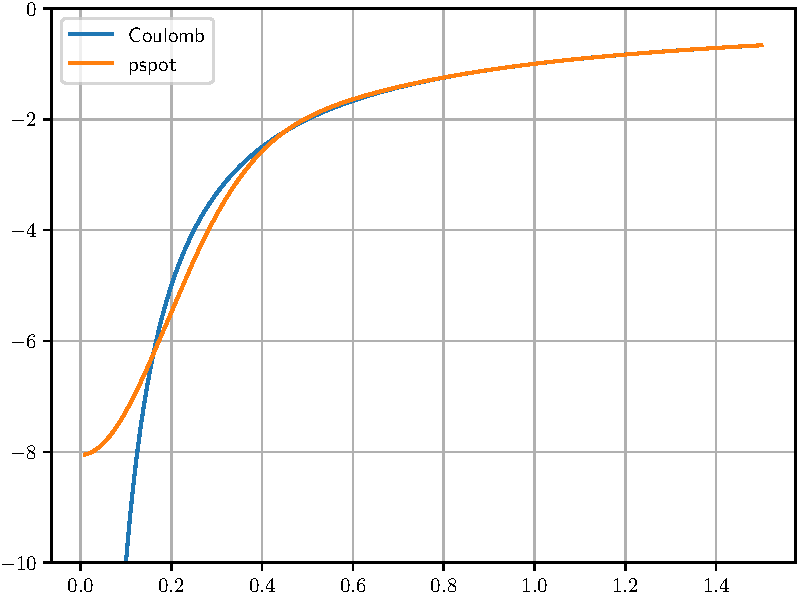
\includegraphics[width=0.65\textwidth]{../codes/sch_3d/IMG_H_Coulomb_vs_pspot.pdf}
\par}
\caption{Comparison Coulomb potential vs pseudopotential}
\label{fig:compare_H_pspot}
\end{figure}

The pseudopotential in \ref{eq:H_psp_GTH} is actually a special case of the more general
form of the local part of pseudopotential developed by Goedecker-Teter-Hutter (GTH):
\begin{equation}
V^{\mathrm{ps}}_{\mathrm{loc}}(r) = -\frac{Z_{\mathrm{val}}}{r}
\mathrm{erf}\left( \frac{\bar{r}}{\sqrt{2}} \right) +
\exp\left( -\frac{1}{2}\bar{r}^2 \right)
\left( C_{1} + C_{2}\bar{r}^2 + C_{3}\bar{r}^4 + C_{4}\bar{x}^6\right)
\label{eq:V_loc_GTH}
\end{equation}
GTH pseudopotentials also come with the nonlocal potential which is considerably more complicated
that the local one.
We will consider the case of nonlocal pseudopotentials in Chapter 7.
GTH pseudopotentials have are parameterized from density functional calculations for many elements
in the periodic table. 



\section{Exercises}

Compare the convergence of eigenvalue of hydrogen potential when using Coulomb potential
vs pseudopotential.

Higher eigenstates of H atom + visualization using Xcrysden

H2 molecule

He atom

LiH molecule